
\documentclass[acmlarge,nonacm=true]{acmart}
\usepackage{adjustbox}
\usepackage{multirow}
\usepackage{graphicx}
\usepackage{afterpage}
\usepackage{subcaption}

\newcommand\blankpage{%
	\null
	\thispagestyle{empty}%
	\addtocounter{page}{-1}%
	\newpage}

%%
%% \BibTeX command to typeset BibTeX logo in the docs
\AtBeginDocument{%
  \providecommand\BibTeX{{%
    \normalfont B\kern-0.5em{\scshape i\kern-0.25em b}\kern-0.8em\TeX}}}


\begin{document}
	
	\begin{titlepage}
		\begin{center}
			\vspace*{1cm}
			
\includegraphics[width=0.7\textwidth]{fig/ntu_logo}
			\vspace{0.8cm}
			\linebreak
			\Huge
			\textbf{Experiment 1: Parametric Curves}
			
			\vspace{0.5cm}
			\LARGE
			CZ2003 Computer Graphics and Visualization
			
			\vspace{1.5cm}
			\textbf{SS3}\\
			
			\begin{table}[h]
				\begin{tabular}{lc}
					Name & Matric Number \\\hline
					Pang Yu Shao & U17216\underline{\textbf{80}}D \\
				\end{tabular}
			\end{table}
			
			
			
			\vfill
			
			\vspace{0.8cm}
			
			
			
			\Large
			SCHOOL OF COMPUTER SCIENCE AND ENGINEERING\\
			NANYANG TECHNOLOGICAL UNIVERSITY\\
			SINGAPORE\\
			2nd Febraury 2021
			
		\end{center}
	\end{titlepage}

 

%%
%% The "title" command has an optional parameter,
%% allowing the author to define a "short title" to be used in page headers.
\title{CZ2003 Computer Graphics and Visualization}

%%
%% The "author" command and its associated commands are used to define
%% the authors and their affiliations.
%% Of note is the shared affiliation of the first two authors, and the
%% "authornote" and "authornotemark" commands
%% used to denote shared contribution to the research.


\author{Pang Yu Shao}
\email{C170134@e.ntu.edu.sg}
\affiliation{\institution{Nanyang Technological University}}

%%
%% By default, the full list of authors will be used in the page
%% headers. Often, this list is too long, and will overlap
%% other information printed in the page headers. This command allows
%% the author to define a more concise list
%% of authors' names for this purpose.
\renewcommand{\shortauthors}{Pang Yu Shao}






%%
%% This command processes the author and affiliation and title
%% information and builds the first part of the formatted document.

% \begin{teaserfigure}
% 	\includegraphics[width=\textwidth]{bccell}
% 	\caption{Breast Cancer Cell. Photograph by National Cancer Institute [Public domain], via Wikimedia
% 		Commons. (\url{https://w.wiki/kS3}).}
% 	\Description{A breast cancer cell seen through an electron microscope.}
% \end{teaserfigure}
% \maketitle



\tableofcontents
\newpage
\section{Defining Surfaces Parametrically}
\subsection{Plane Passing Through Three Defined Points}
To define the plane parametrically, we can use the following formula: \(P = P1+u(P2-P1)+v(P3-P1)\)\\
Therefore, with the 3 points \((N, M, 0),\ (0, M, N),\ (N, 0, M)\), we get:\\
\(x(u,v) = N - Nu = \mathbf{8 - 8u}\)\\
\(y(u,v) = M + Mv = \mathbf{10 + 10v}\)\\
\(z(u,v) = Nu + Mv = \mathbf{8u + 10v}\)\\
\(\mathbf{u,v \in [0,1]}\)

\begin{figure}[H]
	\begin{subfigure}{.33\textwidth}
	  \centering
	  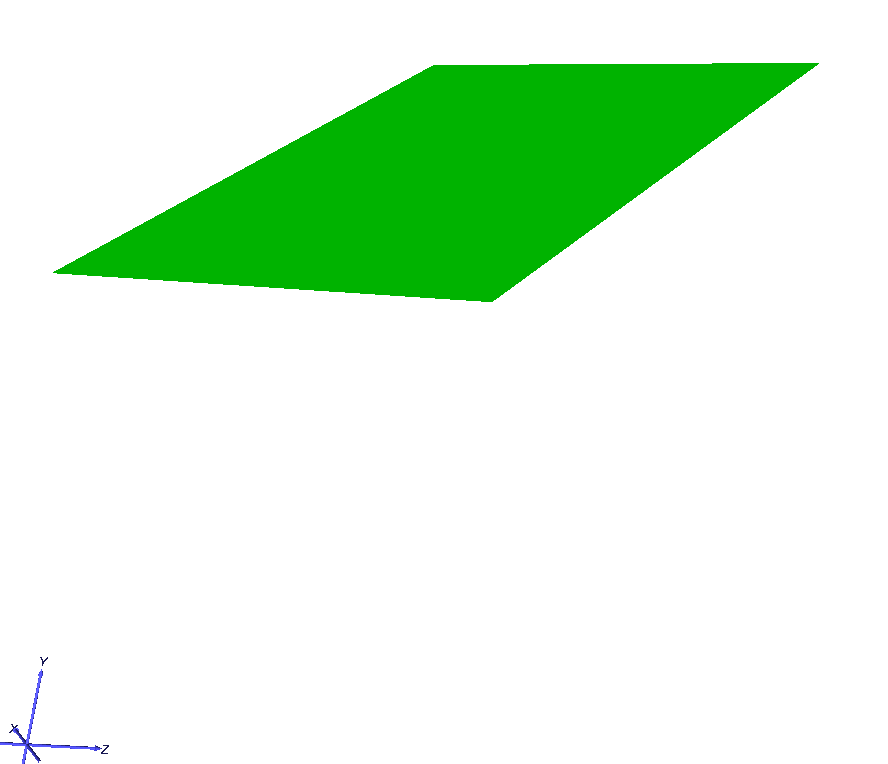
\includegraphics[width=.8\linewidth]{fig/1a1_1}
	  \caption{Resolution: 1 1}
	\end{subfigure}%
	\begin{subfigure}{.33\textwidth}
	  \centering
	  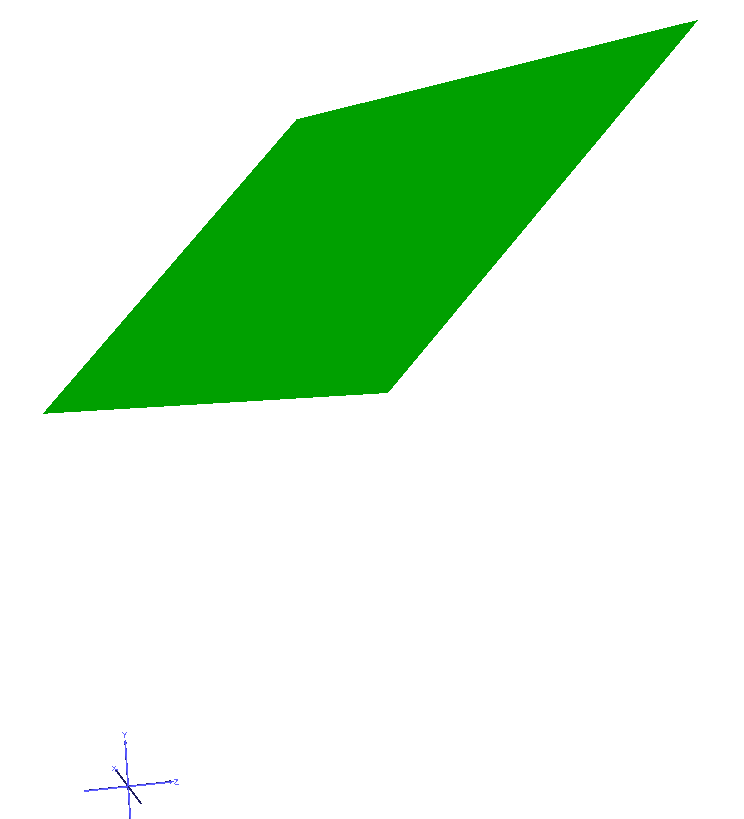
\includegraphics[width=.8\linewidth]{fig/1a10_10}
	  \caption{Resolution: 10 10}
	\end{subfigure}
	\begin{subfigure}{.33\textwidth}
		\centering
		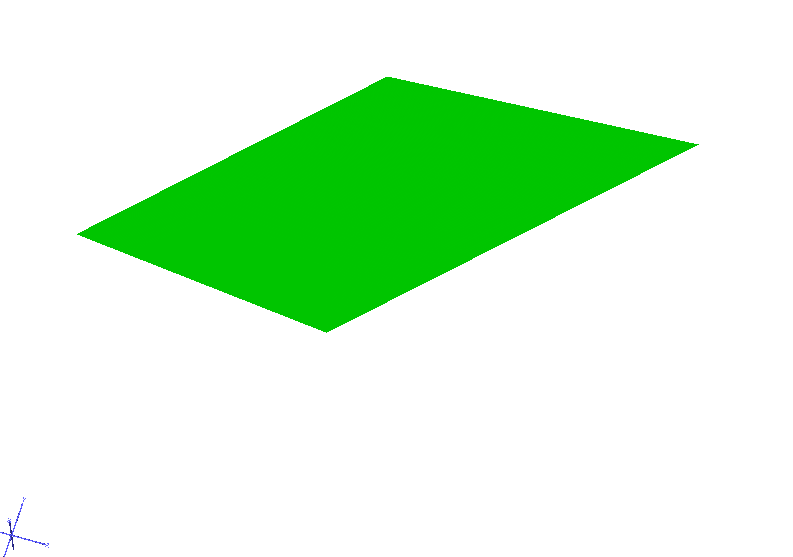
\includegraphics[width=.8\linewidth]{fig/1a1000_1000}
		\caption{Resolution: 1000 1000}
	  \end{subfigure}
	\caption{Plots of the plane defined in "\textbf{1a.wrl}" with differing resolutions}
	\label{fig:1a}
\end{figure}
 
As seen in Fig. \ref{fig:1a} above, a sampling resolution of \textbf{1} for both u and v is 
sufficient for drawing the plane as it has no curvature and having a higher resolution would
produce the exact same drawing.


\bibliographystyle{ACM-Reference-Format}
\newpage





\end{document}
\endinput
%%
%% End of file `sample-acmlarge.tex'.
